\documentclass[letterpaper,12pt]{article}\usepackage[]{graphicx}\usepackage[]{color}
%% maxwidth is the original width if it is less than linewidth
%% otherwise use linewidth (to make sure the graphics do not exceed the margin)
\makeatletter
\def\maxwidth{ %
  \ifdim\Gin@nat@width>\linewidth
    \linewidth
  \else
    \Gin@nat@width
  \fi
}
\makeatother

\definecolor{fgcolor}{rgb}{0.345, 0.345, 0.345}
\newcommand{\hlnum}[1]{\textcolor[rgb]{0.686,0.059,0.569}{#1}}%
\newcommand{\hlstr}[1]{\textcolor[rgb]{0.192,0.494,0.8}{#1}}%
\newcommand{\hlcom}[1]{\textcolor[rgb]{0.678,0.584,0.686}{\textit{#1}}}%
\newcommand{\hlopt}[1]{\textcolor[rgb]{0,0,0}{#1}}%
\newcommand{\hlstd}[1]{\textcolor[rgb]{0.345,0.345,0.345}{#1}}%
\newcommand{\hlkwa}[1]{\textcolor[rgb]{0.161,0.373,0.58}{\textbf{#1}}}%
\newcommand{\hlkwb}[1]{\textcolor[rgb]{0.69,0.353,0.396}{#1}}%
\newcommand{\hlkwc}[1]{\textcolor[rgb]{0.333,0.667,0.333}{#1}}%
\newcommand{\hlkwd}[1]{\textcolor[rgb]{0.737,0.353,0.396}{\textbf{#1}}}%

\usepackage{framed}
\makeatletter
\newenvironment{kframe}{%
 \def\at@end@of@kframe{}%
 \ifinner\ifhmode%
  \def\at@end@of@kframe{\end{minipage}}%
  \begin{minipage}{\columnwidth}%
 \fi\fi%
 \def\FrameCommand##1{\hskip\@totalleftmargin \hskip-\fboxsep
 \colorbox{shadecolor}{##1}\hskip-\fboxsep
     % There is no \\@totalrightmargin, so:
     \hskip-\linewidth \hskip-\@totalleftmargin \hskip\columnwidth}%
 \MakeFramed {\advance\hsize-\width
   \@totalleftmargin\z@ \linewidth\hsize
   \@setminipage}}%
 {\par\unskip\endMakeFramed%
 \at@end@of@kframe}
\makeatother

\definecolor{shadecolor}{rgb}{.97, .97, .97}
\definecolor{messagecolor}{rgb}{0, 0, 0}
\definecolor{warningcolor}{rgb}{1, 0, 1}
\definecolor{errorcolor}{rgb}{1, 0, 0}
\newenvironment{knitrout}{}{} % an empty environment to be redefined in TeX

\usepackage{alltt}
\usepackage[top=1in,bottom=1in,left=1in,right=1in]{geometry}
\usepackage{setspace}
\usepackage[colorlinks=true,urlcolor=blue,citecolor=blue,linkcolor=blue]{hyperref}
\usepackage{indentfirst}
\usepackage{multirow}
\usepackage{booktabs}
\usepackage[final]{animate}
\usepackage{graphicx}
\usepackage{verbatim}
\usepackage{rotating}
\usepackage{tabularx}
\usepackage{array}
\usepackage{subfig} 
\usepackage[noae]{Sweave}
\usepackage{cleveref}
\usepackage[figureposition=bottom]{caption}
\usepackage{paralist}
\usepackage{acronym}
\usepackage{outlines}

%acronyms
\acrodef{doc}[DoC]{depth of colonization}
\acrodef{GIS}{Geographic Information System}

%knitr options


\IfFileExists{upquote.sty}{\usepackage{upquote}}{}
\begin{document}

\setlength{\parskip}{5mm}
\setlength{\parindent}{0in}

\title{Improving spatial resolution in estimates of seagrass depth of colonization}
\author{Marcus W. Beck}
\maketitle

\section{Outline}
\begin{outline}
\1 Needs
\2 Seagrass related to habitat quality and strongly affected by water clarity
\2 Extensive datasets describing historical and current seagrass growth patterns and distribution in Florida estuaries
\2 No consistent approach for estimating \ac{doc} to establish restoration targets
\2 WBID has been considered appropriate management unit although considerable spatial heterogeneity in seagrass growth
\2 Reproducible and empirical approaches can be developed that leverage multiple types of information to provide more consistent estimates for restoration targets or nutrient criteria
\1 Objectives
\2 Use information-rich datasets to estimate seagrass \ac{doc} by incorporating spatially referenced information
\2 Provide a basis for using these estimates to inform nutrient criteria development using empirical relationships with water clarity
\1 Approach
\2 Describe Hagy method and/or WBID approach, emphasis on situations where seagrass growth is spatially variable or when restoration target is misinformed
\2 Describe spatially-referenced method, case studies
\2 Compare/contrast the two, with emphasis on relation to secchi data
\2 Implications for criteria development and/or restoration targets
\1 To do
\2 Rectify seagrass depth bin procedures
\2 Tidal datum correction
\2 Segment specific relationship of seagrass depth of col w/ Secchi
\2 Compare cumulative sum approach with binning
\2 Quantitative evaluation of grid spacing, grid location, and radius
\end{outline}

\section{Methods}

The following describes methods used to estimate seagrass \ac{doc} that incorporate spatial information to improve resolution.  Methods build extensively on those in Hagy et al. (in prep).  

\subsection{Significant within-segment variation in seagrass depth of colonization}

First, an example is provided that illustrates spatial heterogeneity within an individual estuary segment to highlight a need for improved resolution.  These segments are commonly used as a basis for quantifying nutrient criteria and it is shown that these spatial scales  may not be sufficient for characterizing variation in seagrass growth. Hagy et al. (in prep) describe methods for estimating seagrass \ac{doc} by segments using historical and current records of seagrass coverage combined with bathymetric data.  The approach begins by combining bathymetric sounding data with coverage data to create a \ac{GIS} layer containing both sets of information.  The points are groups into depth bins and the proportion of points within each depth bin that contain seagrass are quantified.  The maximum \ac{doc} for each segment is estimated using a plot of proportion of points occupied against depth bin.  In general, the plot is characterized by a decreasing trend such that the proportion of occupied points by depth bin decreases and flattens with increasing depth.  A regression is fit on this descending portion such that the intercept point on the x-axis is considered the maximum depth of colonization.  The median portion of this curve is considered the median depth of the deepwater edge of seagrass.  Estimates are obtained for seagrass coverage layers that describe continuous and continuous with patchy seagrass.  

\cref{Fig:wbid_doc} illustrates spatial variation in seagrass distribution on a latitudinal gradient in Old Tampa Bay, Florida.  The estimate for median seagrass \ac{doc} for the entire segment is an over- and under-estimate for northern and southern portions, respectively.  This suggests that estimates of \ac{doc} are needed at finer spatial scales to provide a more robust determination of restoration targets and nutrient criteria. 

\subsection{Estimating seagrass depth of colonization using spatial information}

Regression approach vs cumulative distribution

\subsection{Sensitivity analysis and comparison with segment-based approach}

\subsection{Developing a spatially coherent relationship of water clarity with depth of colonization}

%%%%%%
% figures
\clearpage

%%%%%%
% example of depth of col ests for wbid
\begin{figure}
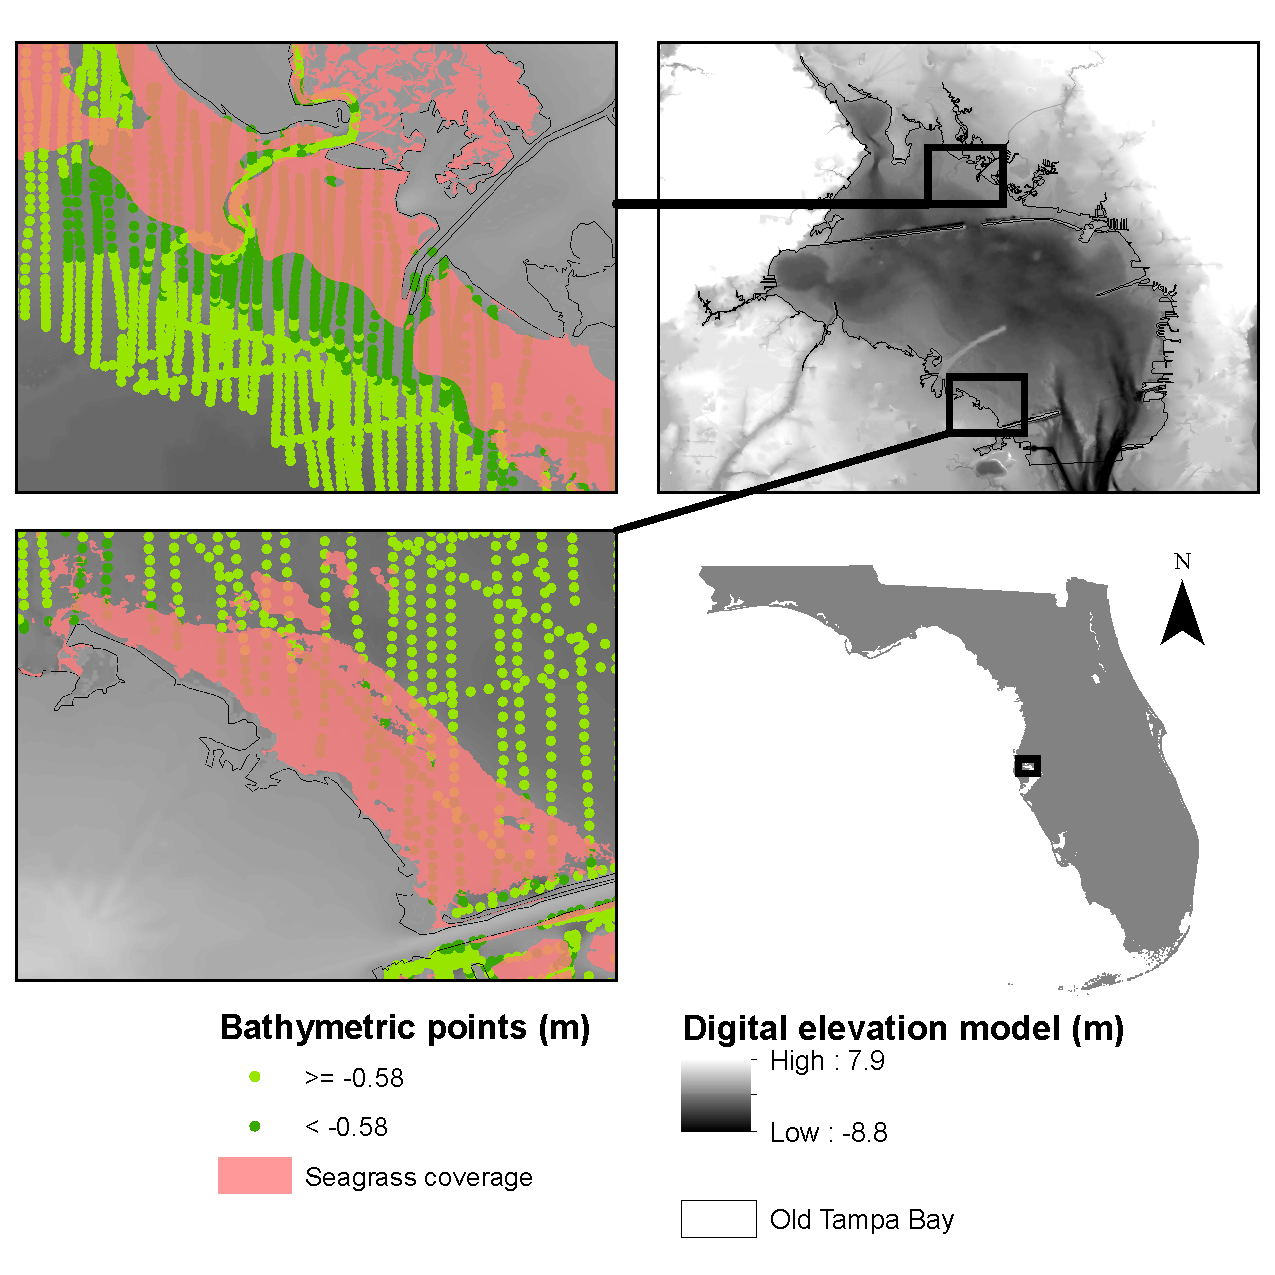
\includegraphics[width = \textwidth]{figs/wbid_doc.pdf}
\caption{Example of over- and under-estimates for seagrass depth of colonization in Old Tampa Bay, Florida.  The top-left figure indicates over-estimation and the bottom-left indicates under-estimation.  Bathymetric points are color-coded by the median depth of colonization estimate for all seagrass (patchy and continuous) in the segment.}
\label{fig:wbid_doc}
\end{figure}

\end{document}
